\section{Composition Filters in \Compose*{}}
\label{sec:CompositionFiltersInComposeStar}

% Removed "t" so that it is not longer breaking the history list
\begin{lstlisting}[language=Composestar,style=floatlisting,float=bp, caption={Abstract concern template},label={lst:concerntemplate}]
concern {
  filtermodule {
    internals
    externals
    conditions
    inputfilters
    outputfilters
  }
  
  superimposition {
    selectors
    filtermodules
    annotations
    constraints
  }
  
  implementation
}
\end{lstlisting}

A \Compose* application consists of concerns that can be divided in three parts: filter module specifications, superimposition, and implementation.
A filter module contains the filter logic to filter on incoming or outgoing messages on superimposed objects.
Messages have a target, which is an object reference, and a selector, which is a method name.
A superimposition part specifies which filter modules, annotations, conditions, and methods are superimposed on which objects.
An implementation part contains the class implementation of a concern.
How these parts are placed in a concern is shown in \autoref{lst:concerntemplate}.

\begin{figure}[htbp]
  \centering
  \includegraphics[style=thirdheight]{cfmodel}
  \caption{Components of the composition filters model}
  \label{fig:cfmodel}
\end{figure}

The working of a filter module is depicted in \autoref{fig:cfmodel}.
A filter module can contain input and output filters.
The difference between these two sets of filters is that the first is used to filter on incoming messages, while the second is used to filter on outgoing messages.
The return of a method is not considered an outgoing message.
A filter has three parts: a filter identifier, a filter type, and one or more filter elements.
A filter element exists out of an optional condition part, a matching part, and a substitution part.
These parts are shown below:
\begin{center}
$\overbrace{stalker\_filter}^{identifier}:\overbrace{Dispatch}^{filter~type}~=~\{\overbrace{!pacmanIsEvil}^{condition~part}
=>\overbrace{[*.getNextMove]}^{matching~part}~\overbrace{stalk\_strategy.getNextMove}^{substitution~part}~\}$
\end{center}
A filter identifier is a unique name for a filter in a filter module. 
Filters match when both the condition part and the matching part evaluate to true.
In the demonstrated filter, every message where the selector is \lstinline|getNextMove| matches.
If an asterisk~(\lstinline|*|) is used in the target, every target will match.
When the condition part and the matching part are true, the message is substituted with the values provided in the substitution part.
How these values are substituted, and how the message continues, depends on the type of filter used.
At the moment there are four basic filter types defined in \Compose*.
It is, however, possible to write custom filter types.

\begin{description}[style=sameline,leftmargin=18mm]
  \item[Dispatch] If the message is accepted, it is dispatched to the specified target of the message, otherwise the message continues to the subsequent filter.
    This filter type can only be used for input filters;
  \item[Send] If the message is accepted, it is sent to the specified target of the message, otherwise the message continues to the subsequent filter.
    This filter type can only be used for output filters;
  \item[Error] If the filter rejects the message, it raises an exception, otherwise the message continues to the next filter in the set;
  \item[Meta] If the message is accepted, the message is sent as a parameter of another meta message to an internal or external object, otherwise the message just continues to the next filter.
    The object that receives the meta message can observe and manipulate the message and can re-activate the execution of the message.
\end{description}

The identifier \lstinline|pacmanIsEvil|, used in the condition part, must be declared in the conditions section of a filter module.
Targets that are used in a filter can be declared as internal or external.
An internal is an object that is unique for each instance of a filter module, while an external is an object that is shared between filter modules.

Filter modules are superimposed on classes using filter module binding, which specifies a selection of objects on the one side, and a filter module on the other side.
The selection is specified in a selector definition.
This selector definition uses predicates to select objects, such as \lstinline|isClassWithNameInList|, \hbox{\lstinline|isNamespaceWithName|}, and \lstinline|namespaceHasClass|.
In addition to filter modules, it is possible to bind conditions, methods, and annotations to classes using superimposition.

The last part of the concern is the implementation part, which can be used to define the behavior of a concern.
For a logging concern, for example, we can define specific log functions and use them as internal.

